\chapter{Crittografia Post-Quantum}

\begin{citazione}
    Questo capitolo ha lo scopo di introdurre brevemente gli strumenti crittografici utilizzati, ponendo particolare enfasi anche sui concetti sui quali sono costruiti questi strumenti.
\end{citazione}

\section{Problema dei computer quantistici}
Un \emph{computer quantistico} è un elaboratore che, a differenza di un "classico" computer basato su \emph{transistor}, sfrutta la \emph{meccanica quantistica} per svolgere operazioni sui dati. In particolare, sfrutta le \emph{proprietà quantistiche} della materia (come ad esempio la sovrapposizione degli stati) e per questa ragione non utilizza come \emph{unità base di informazione} i \textbf{bit} per rappresentare lo stato della materia ma i \textbf{qubit}, simile ai \emph{bit} ma con la caratteristica di poter essere anche in due stati contemporaneamente (non come i bit che possono avere o solo valore 0 o solo 1). Questo perchè lo stato della materia (dal punto di vista quantistico) non sempre è in un solo stato e, quindi, per rispecchiare questa caratteristica è stato introdotto il \emph{qubit}. \cite{wikipedia_quantum_computing}

Utilizzando un'architettura completamente diversa, è stato teorizzato un modello computazionale che descriva in maniera astratta un computer quantistico: la \textbf{Macchina di Turing quantistica}. Questa ha la caratteristica di essere equivalente ad una \textbf{Macchina di Turing} classica dal punto di vista del potere computazionale, tuttavia dal punto di vista delle "\textbf{prestazioni}" sembra che la macchina \emph{quantistica} sia molto più veloce di una macchina classica e, nella pratica, si traduce in elaboratori che sono molto più veloci dei normali computer diventando una vera e propria minaccia per la sicurezza dei sistemi. Infatti, esiste un algoritmo chiamato \textbf{Algoritmo di Shor} che, se eseguito su un computer quantistico abbastanza potente, permette di risolvere dei problemi che sono "\textbf{difficili}" per un normale computer in tempo \emph{polinomiale} (tempo molto breve), ovvero eseguire la fattorizzazione di un numero intero e il calcolo del logaritmo discreto, i quali sono i \textbf{problemi} su cui si basano rispettivamente il cifrario \textbf{RSA} e il cifrario \textbf{ElGamal} e sono attualmente gli schemi crittografici più utilizzati. Tuttavia, per utilizzare questo algoritmo in maniera efficace c'è bisogno di un computer quantistico in grado di utilizzare un numero di \textbf{qubit} abbastanza alto e per il momento ancora non esistono computer del genere, ma ciò non toglie che in futuro possa essere realizzato ed essere in grado di \emph{rompere} tutti i cifrari conosciuti basati sui problemi citati in precedenza. \cite{wikipedia_quantum_computing}

Al fine di correre subito ai ripari, il \textbf{NIST} (National Institute of Standards and Technology) ha subito aperto un \emph{concorso} aperto a chiunque con lo scopo di standardizzare degli algoritmi a chiave pubblica in grado di \textbf{resitere all'attacco di un computer quantistico}, quindi che non sono basati su un problema risolvibile dall'\emph{algoritmo di Shor}. Questi algoritmi prendono il nome di \textbf{Crittografia Post-Quantistica} e sono tutti basati su problemi che non sono risolvibili in maniera facile nemmeno da un computer quantistico. \cite{wikipedia_quantum_computing}


\section{\emph{KEM}}
Un \textbf{Key Encapsulation Mechanism} è un algoritmo a chiave pubblica che permette di inviare in maniera sicura un segreto condiviso ad un interlocutore. Solitamente un \emph{KEM} tra due interlocutori \textbf{A} e \textbf{B} funziona nel seguente modo:
\begin{enumerate}
    \item \textbf{A} prende la chiave pubblica di \textbf{B} e la usa per generare il segreto da inviare (che custodirà in maniera sicura) e una \emph{capsula} che contiene il segreto in maniera "cifrata";
    \item \textbf{A} invia la \emph{capsula} a \textbf{B};
    \item \textbf{B} utilizza la sua chiave privata per aprire la \emph{capsula} e leggere il segreto inviato da \textbf{A}.
\end{enumerate}

Un \emph{KEM} può essere anche definito come un insieme di tre algoritmi:
\begin{itemize}
    \item \texttt{Gen(n)}: prende in input \texttt{n}, anche detto parametro di sicurezza (definisce quanto devono essere lunghe le chiavi generate), e restituisce una coppia di chiavi \texttt{pk} e \texttt{sk}, rispettivamente pubblica e privata;
    \item \texttt{Encaps(pk)}: prende in input la chiave pubblica \texttt{pk} e restituisce un segreto \texttt{ss} e il relativo testo cifrato \texttt{ct} (la \emph{capsula});
    \item \texttt{Decaps(ct, sk)}: prende in input la \emph{capsula} \texttt{ct} e la chiave privata \texttt{sk} e restituisce il segreto \texttt{ss}.
\end{itemize}

L'utilizzo più diffuso di un \emph{KEM} è quello di scambiare una chiave di sessione all'interno di un \textbf{cifrario ibrido}, ovvero uno schema di cifratura che utilizza sia una parte \textbf{asimmetrica} che una \textbf{simmetrica}, quindi il \emph{segreto} che viene incapsulato è un valore totalmente casuale (generato ad ogni chiamata di \texttt{Encaps()}) che viene utilizzato come chiave. Tuttavia, è possibile modificare leggermente l'algoritmo \texttt{Encaps()} facendogli prendere in input anche un secondo valore \texttt{ss} scelto arbitrariamente, in modo tale da permettere anche uno \textbf{scambio di messaggi} e non solo uno \textbf{scambio di chiavi}. Un esempio di \emph{KEM} che può essere utilizzato in questo modo è \textbf{RSA}, che permette di scambiare sia chiavi che messaggi in modo da adattarsi a più utilizzi. \cite{wikipedia_kem}

\section{CRYSTALS-kyber}
Uno dei tanti algoritmi \emph{Post-Quantum} disponibili è l'algoritmo \textbf{CRYSTALS-kyber}, un \emph{KEM} che basa la sua sicurezza su un problema noto per essere difficile anche per un elaboratore quantistico. L'algoritmo si presenta in tre versioni, ognuna delle quali si differenzia per il \emph{parametro di sicurezza} (lunghezza della chiave) e al "livello" di sicurezza in grado di garantire. Facendo un parallelo con il noto algoritmo di cifratura \textbf{AES}, prendendo in considerazione solo il livello di sicurezza garantito, si può dire che \textbf{kyber-512} offre un livello di sicurezza comparabile con \textbf{AES-128}, \textbf{kyber-768} con \textbf{AES-192} e \textbf{kyber-1024} con \textbf{AES-256}. \cite{kyber}

Sebbene offra un ottimo livello di sicurezza, le prestazioni ne risentono in maniera abbastanza evidente. Infatti, nell'ipotesi di uno scenario di cifratura di una chat, utilizzando un algortimo \textbf{non-quantum-safe} (non resistente all'attacco di un computer quantistico) come \textbf{ECDH} (Elliptic-Curve Diffie-Hellman, un \emph{KEM} basato sul problema del logaritmo discreto) si può notare che è 2 volte più veloce, consuma circa 2 volte meno energia e genera un overhead sui dati circa 70 volte inferiore rispetto a \textbf{kyber}. \cite{wikipedia_kyber}

\subsection{Sicurezza del cifrario}
Un cifrario, per essere considerato sicuro, deve possedere la proprietà di \textbf{indistinguibilità}, ovvero preso un \emph{testo cifrato} non deve essere possibile stabilire a quale \emph{testo in chiaro} corrisponda. Persa questa proprietà è ovvio che uno schema non può essere considerato sicuro in quanto è sempre possibile risalire al corrispondente \emph{testo in chiaro} senza conoscere la chiave di cifratura.

Il modello che di solito si utilizza per dimostrare la sicurezza di un cifrario è un gioco dove un avversario ha due messaggi in chiaro e un testo cifrato corrispondente ad uno dei due messaggi. L'obiettivo dell'avversario, ovviamente, è quello di indovinare il testo in chiaro corrispondente e nel farlo può avere a disposizione più o meno potere computazionale per cercare di indovinarlo, come ad esempio la possibilità di ottenere dei testi cifrati a partire da testi in chiaro a piacere (ovviamente che non fanno parte dei messaggi in chiaro della sfida). Se l'avversario, grazie al potere a disposizione, è in grado di stabilire l'origine del testo cifrato con una buona probabilità, allora il cifrario \textbf{non è sicuro contro quell'avversario}, mentre se l'avversario non riesce ad estrapolare informazioni e l'unica cosa che riesce a fare è tentare a caso, allora \textbf{il cifrario è sicuro contro quell'avversario}. In base al potere fornito all'avversario si possono identificare tre livelli di sicurezza:  

\begin{enumerate}
    \item \textbf{IND-CPA} (\emph{Chosen-Plaintext Attack}): l'attaccante ha accesso ad un \textbf{oracolo di cifratura} che gli permette di ottenere il corrispondente \emph{testo cifrato} a partire da \emph{testi in chiaro} a piacere che non siano quelli della sfida. Ovviamente l'oracolo utilizza la stessa chiave utilizzata per cifrare il \emph{testo cifrato} della sfida e l'avversario non la conosce perchè l'oracolo lavora come una \textbf{scatola chiusa};
    \item \textbf{IND-CCA1} (\emph{Chosen-Ciphertext Attack}): oltre ad avere accesso all'\textbf{oracolo di cifratura}, l'attaccante ha anche accesso ad un \textbf{oracolo di decifratura} che gli permette di decifrare (sempre con la chiave utilizzata per la sfida) \emph{testi cifrati} arbitrari. Tuttavia, nel momento in cui riceve il \emph{testo cifrato} di sfida, non può più utilizzare l'\textbf{oracolo di decifratura} e deve scegliere uno dei due testi in chiaro di sfida;
    \item \textbf{IND-CCA2} (\emph{adaptive Chosen-Ciphertext Attack}): nella versione \emph{adattiva}, l'unica differenza rispetto alla precedente è che adesso l'avversario può utilizzare l'\textbf{oracolo di decifratura} anche dopo aver ricevuto il \textbf{cifrato di sfida}.
\end{enumerate}

È chiaro che l'avversario \textbf{IND-CCA2} è il più potente mentre l'avversario \textbf{IND-CPA} è il meno potente e, ovviamente, se un cifrario è sicuro nei confronti di un avversario con un certo potere sarà sicuro anche per quelli con potere minore. \cite{wikipedia_cipher_security}\\
Per quanto riguarda il cifrario \textbf{CRYSTALS-kyber}, è stato dimostrato essere \textbf{IND-CCA2}-sicuro, per cui è in grado di resistere anche agli attacchi più sofisticati e agli attaccanti più potenti. \cite{kyber}

\subsection{Problema di riferimento}
Il problema su cui si basa il cifrario \textbf{CRYSTALS-kiber} è chiamato \textbf{Learning With Errors} (\emph{LWE}), appartenente alla famiglia dei problemi \textbf{lattice-based} (basati sui reticoli ordinati). Sebbene sia un problema algebrico abbastanza complesso, l'idea di base è molto semplice: dato un sistema di equazioni lineari che descrivono il valore del segreto da condividere, questo si può nascondere aggiungendo degli errori al sistema. In questo modo, un sistema risolvibile in maniera facile diventa risolvibile in maniera difficile persino per un computer quantistico, anche con degli \textbf{errori piccoli}.\\
Tipicamente per rendere più efficiente la risoluzione del sistema vengono introdotti dei \textbf{numeri interi} come \emph{errori}, in quanto le operazioni necessarie per la risoluzione sono implementabili in maniera molto efficiente. Un esempio di sistema a cui vengono aggiunti errori può essere visualizzato in \autoref{fig:lwe-example} \cite{telsy_lwe}

\begin{figure}[h]
    \begin{subfigure}{0.4\textwidth}
        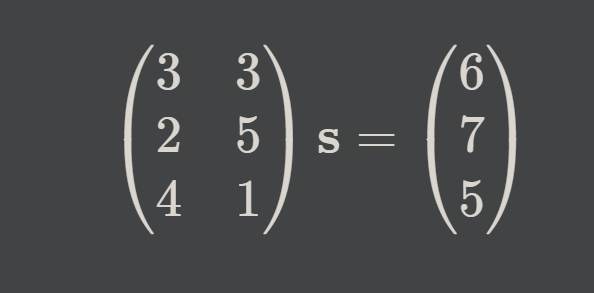
\includegraphics[width=1\textwidth]{capitoli/figure-crittografia/lwe-no-error.png}
    \end{subfigure}
    \hfill
    \begin{subfigure}{0.5\textwidth}
        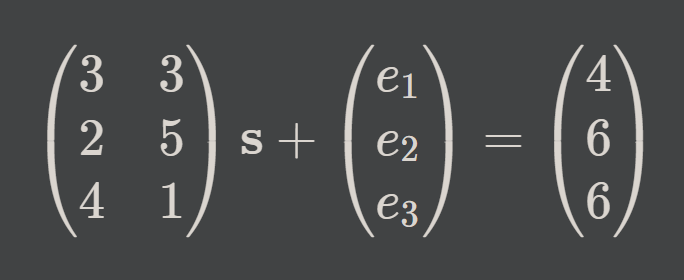
\includegraphics[width=1\textwidth]{capitoli/figure-crittografia/lwe-with-error.png}
    \end{subfigure}
    \caption{Esempio di sistema senza errori (sinistra) e lo stesso ma con l'aggiunta di errori (destra)}
    \label{fig:lwe-example}
\end{figure}

Il fatto che sia complesso anche per un computer quantistico deriva dal fatto che questo problema è possibile ridurlo ad un altro problema già noto essere difficile per un computer quantistico. Il problema in questione è il \textbf{CVP} (Closest Vector Problem) che è definito su una struttura geometrica chiamata reticolo, un insieme di punti che può essere descritto come una \textbf{griglia}. In pratica, definiti due o più vettori di base, il reticolo risultante è un insieme di "punti" ottenuti facendo combinazioni lineari \textbf{intere} (che utilizzano solo numeri interi) di questi vettori. Alcuni esempi di reticoli possono essere visti in \autoref{fig:lattice-examples}

\begin{figure}[h]
    \begin{subfigure}{0.48\textwidth}
        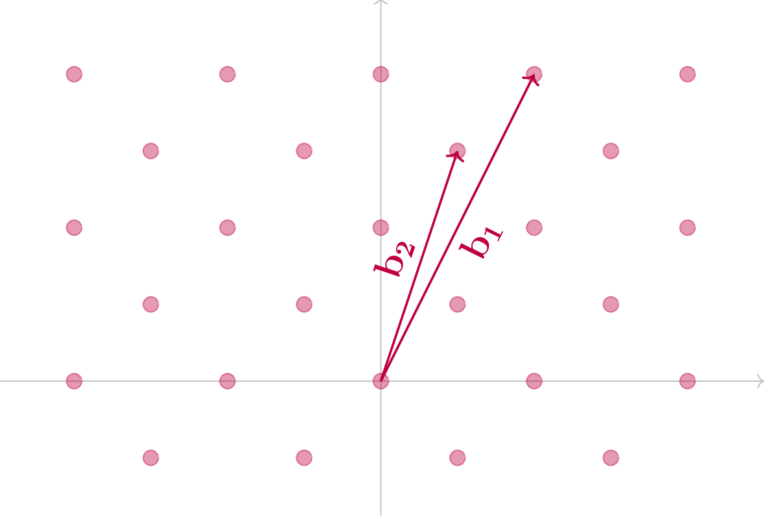
\includegraphics[width=1\textwidth]{capitoli/figure-crittografia/lattice-2.png}
        \caption{Esempio di reticolo a due dimensioni}
    \end{subfigure}
    \hfill
    \begin{subfigure}{0.48\textwidth}
        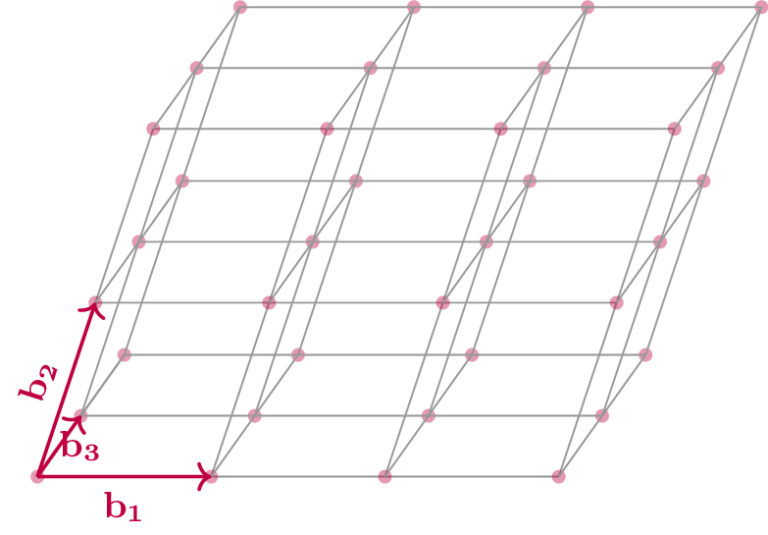
\includegraphics[width=1\textwidth]{capitoli/figure-crittografia/lattice-3.png}
        \caption{Esempio di reticolo a tre dimensioni}
    \end{subfigure}
    \caption{Alcuni esempi di reticoli}
    \label{fig:lattice-examples}
\end{figure}

A questo punto, il problema \textbf{CVP} consiste nel trovare il vettore del reticolo più vicino ad un vettore target definito all'esterno del reticolo. Come si può vedere in \autoref{fig:lattice-cvp}, i punti rossi sono i vettori del reticolo, il vettore blu \texttt{t} è il vettore target definito \textbf{all'esterno} del reticolo e il punto \texttt{x} è il vettore \textbf{del reticolo} più vicino al vettore \texttt{t}. \cite{telsy_lattice}

\begin{figure}[h]
    \centering
    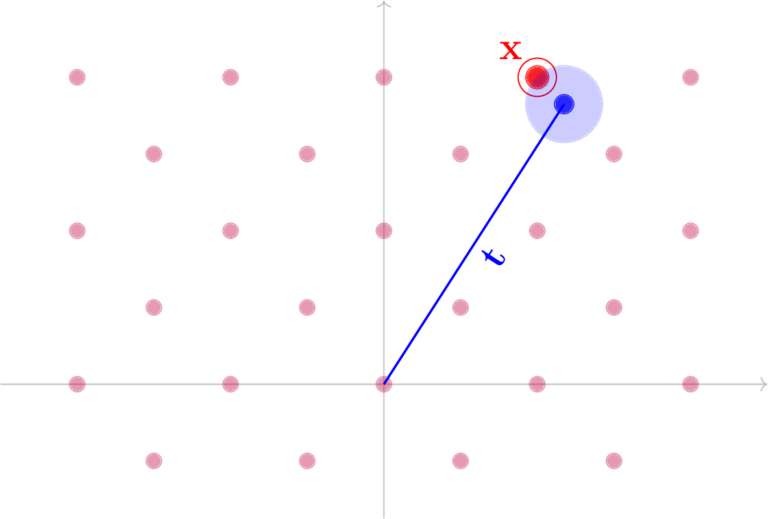
\includegraphics[width=0.9\textwidth]{capitoli/figure-crittografia/lattice-cvp.png}
    \caption{Esempio di problema \emph{CVP}}
    \label{fig:lattice-cvp}
\end{figure}

Questo problema è molto semplice quando le dimensioni del reticolo sono due, tuttavia, se si prende in considerazione un reticolo con \texttt{n} dimensioni il problema diventa molto difficile e nemmeno la potenza di un computer quantistico consente di risolvere il problema in maniera efficiente \cite{hwupgrade_kyber}.

\section{Advanced Encryption Standard}
Con il termine \textbf{AES} si intende la specifica per la protezione dei dati digitali stabilita dal \textbf{NIST} nel 2001 a seguito della volontà di voler sostituire \textbf{DES} (Data Encryption Standard), lo standard utilizzato fino a quel momento. Per definire l'algoritmo \textbf{AES} il \textbf{NIST} ha avviato un concorso aperto a chiunque dove si poteva proporre un algoritmo che doveva rispettare i requisiti imposti dall'ente. Al termine di questo concorso l'algoritmo vincitore è stato il \textbf{Rijndael}, un cifrario a blocchi che si presenta in tre versioni differenziate principalmente dalla lunghezza della chiave (e quindi dal livello di sicurezza che vogliono garantire).

Sostanzialmente un \textbf{cifrario a blocchi} è un \textbf{cifrario a chiave simmetrica} che non opera su un byte alla volta ma organizza il dato da cifrare in gruppi della stessa lunghezza e opera su un intero gruppo alla volta. Nel caso di \emph{AES}, l'input viene suddiviso in gruppi di 128 bit e laddove la lunghezza dell'input non dovesse essere un multiplo di 128 viene aggiunto un \emph{padding} per riempire l'ultimo blocco.\\
Il vantaggio di utilizzare un \textbf{cifrario a blocchi} piuttosto che uno \textbf{stream cipher} (cifrario che cifra un bit alla volta invece che a gruppi), è la possibilità di implementarlo realizzando una struttura chiamata \textbf{rete a sostituzione e permutazione} (\emph{SP-network}) \cite{wikipedia_aes} con la quale si possono facilmente garantire due caratteristiche \emph{chiave} di ogni cifrario:
\begin{itemize}
    \item \textbf{Confusione}: un cifrario dovrebbe fare in modo che ogni bit del testo cifrato deve dipendere da più bit della \textbf{chiave di cifratura}, in modo da oscurare quanto più possibile la relazione tra le due;
    \item \textbf{Diffusione}: un cifrario dovrebbe fare in modo che nel momento in cui cambia un singolo bit del testo in chiaro devono cambiare almeno la metà dei bit del testo cifrato, in modo tale da nascondere quanto più possibile le relazioni statistiche tra testo in chiaro e testo cifrato. \cite{wikipedia_confusion}
\end{itemize}

Il modo in cui si possono garantire queste proprietà è per mezzo dell'introduzione di due particolari strutture all'interno dell'algoritmo:
\begin{itemize}
    \item \textbf{S-box} (Substitution box): è una tabella che definisce come ogni sequenza di una determinata lunghezza deve essere sostituita. Una tipica \emph{S-box} prende un byte, lo divide in due gruppi di 4 bit (chiamati solitamente \textbf{nibble}) e utilizza le due metà per identificare riga e colonna di una tabella. Il byte contenuto nella cella sarà quello che sostiuirà il byte iniziale. Grazie a questa è possibile introdurre la \textbf{confusione}, in quanto quello che vuole realizzare una \emph{S-box} è una relazione \textbf{non-lineare} tra input e output; \cite{wikipedia_s-box}
    \item \textbf{P-box} (Permutation box): è un tabella che definisce come devono essere permutati i bit di un una sequenza fornita in input. Grazie a questa è possibile introdurre la \textbf{diffusione}. \cite{wikipedia_p-box}
\end{itemize}

Un esempio di \textbf{P-box} può essere visto in \autoref{fig:aes-p-box} mentre un esempio di \textbf{S-box} in \autoref{fig:aes-s-box}


\begin{figure}[h]
    \begin{subfigure}{0.48\textwidth}
        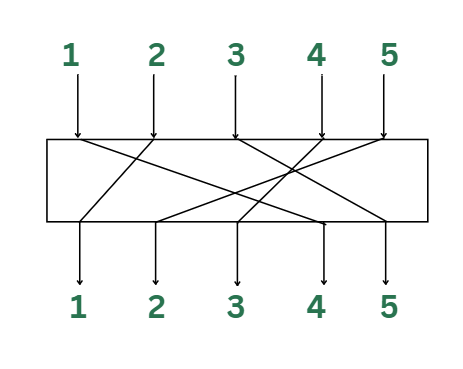
\includegraphics[width=1\textwidth]{capitoli/figure-crittografia/p-box.png}
        \caption{Esempio di una \textbf{P-box}}
        \label{fig:aes-p-box}
    \end{subfigure}
    \hfill
    \begin{subfigure}{0.48\textwidth}
        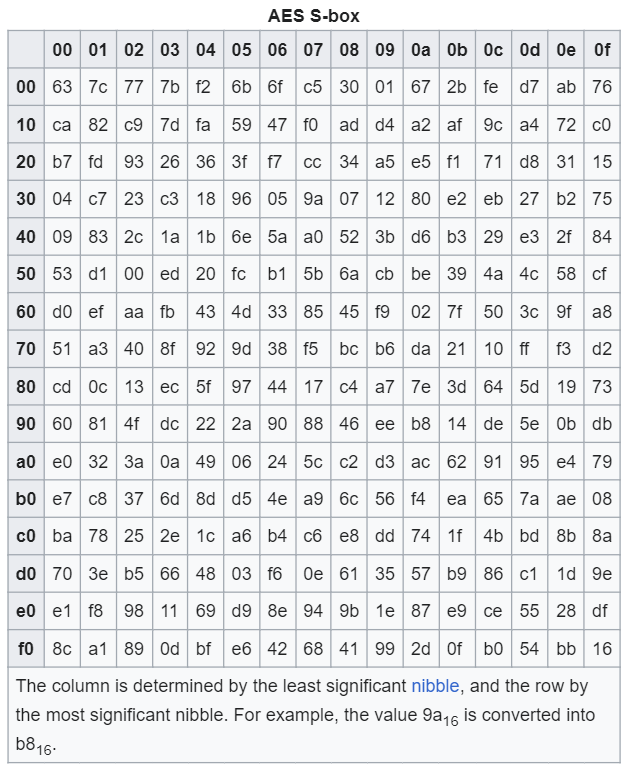
\includegraphics[width=1\textwidth]{capitoli/figure-crittografia/aes-s-box.png}
        \caption{\textbf{S-box} utilizzata dall'algoritmo \emph{Rijndael}}
    \label{fig:aes-s-box}
    \end{subfigure}
    \caption{Esempio di \textbf{S-box} e \textbf{P-box}}
    \label{fig:aes-boxes}
\end{figure}

\subsection{Struttura di \emph{AES}}
L'algoritmo \emph{Rijndael} è stato progettato seguendo lo schema di una \textbf{rete a sostituzione e permutazione} con dimensione del blocco fissa a 128 bit e lunghezza della chiave che può essere lunga 128 bit, 192 bit o 256 bit. La dimensione della chiave influisce sul \textbf{numero di round} (cicli) che vengono eseguiti sul testo in chiaro per generare il testo cifrato finale (la corrispondenza è illustrata in \autoref{table:aes-rounds}).

\begin{table}[h]
    \centering
    \begin{tabular}{| c | c |}
        \hline
        \textbf{Lunghezza chiave} & \textbf{Numero di round} \\
        \hline
        128 & 10 \\
        \hline
        192 & 12 \\
        \hline
        256 & 14 \\
        \hline
    \end{tabular}
    \caption{Numero di round predefinito in \emph{AES}}
    \label{table:aes-rounds}
\end{table}

Il primo passo che esegue l'algoritmo è un espansione della chiave in modo da ottenere le chiavi da utilizzare per ogni round, mentre ogni round è composto principalmente da 4 operazioni: \texttt{SubBytes}, \texttt{ShiftRows}, \texttt{MixColumns} e \texttt{AddRoundKey}.

\subsubsection{SubBytes}
Lo scopo di questa operazione è quella di realizzare una sostituzione \textbf{non lineare} dei byte, per mezzo delle \textbf{S-box}, in modo da introdurre \textbf{confusione} ed evitare banali attacchi algebrici. Una visualizzazione dell'operazione può essere vista in \autoref{fig:aes-subbytes}. \cite{wikipedia_aes}

\begin{figure}[h]
    \centering
    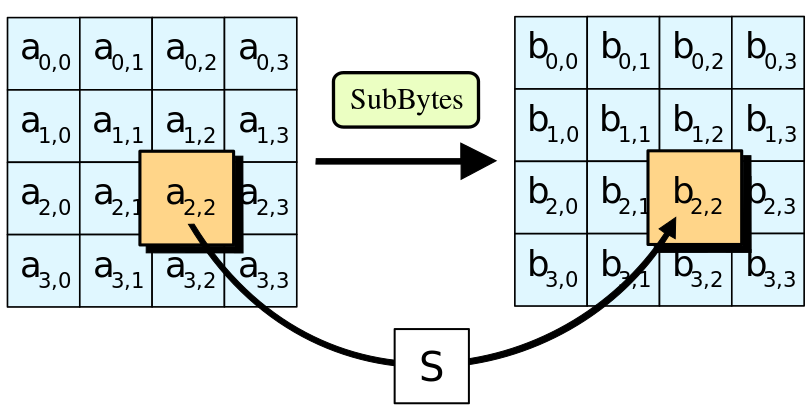
\includegraphics[width=0.6\textwidth]{capitoli/figure-crittografia/aes-SubBytes.png}
    \caption{Schema dell'operazione \emph{SubBytes}}
    \label{fig:aes-subbytes}
\end{figure}

\subsubsection{ShiftRows}
Lo scopo di questa operazione è quella di effettuare lo \textbf{shift} di ogni riga di un determinato offset, in modo da non cifrare le colonne in maniera indipendente degenerando in 4 cifrari a blocchi indipendenti (si introdurrebbe una problematica simile a quella affrontata nella \autoref{section:aes-modes} con la modalità \emph{ECB}). In generale l'offset è 0 per la prima riga (rimane invariata) e aumenta di 1 ad ogni riga successiva, in questo modo ogni colonna conterrà byte appartenenti ad ogni altra colonna. Una visualizzazione dell'operazione può essere vista in \autoref{fig:aes-shiftrows}. \cite{wikipedia_aes}

\begin{figure}[h]
    \centering
    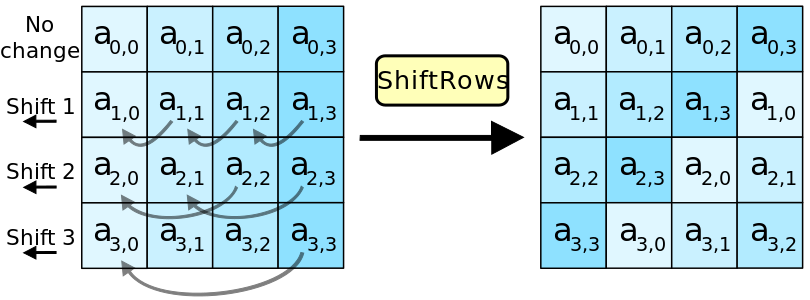
\includegraphics[width=0.6\textwidth]{capitoli/figure-crittografia/aes-ShiftRows.png}
    \caption{Schema dell'operazione \emph{ShiftRows}}
    \label{fig:aes-shiftrows}
\end{figure}

\subsubsection{MixColumns}
Lo scopo di quest'operazione è quella di combinare le varie colonne in maniera \textbf{lineare} e \textbf{reversibile}, facendo in modo che la combinazione dei 4 byte della colonna influiscano \textbf{sempre} su ogni byte della colonna di output. Insieme all'operazione di \textbf{ShiftRows}, quest'operazione introduce la \textbf{diffusione}. Una visualizzazione dell'operazione può essere vista in \autoref{fig:aes-mixcolumns}. \cite{wikipedia_aes}

\begin{figure}[h]
    \centering
    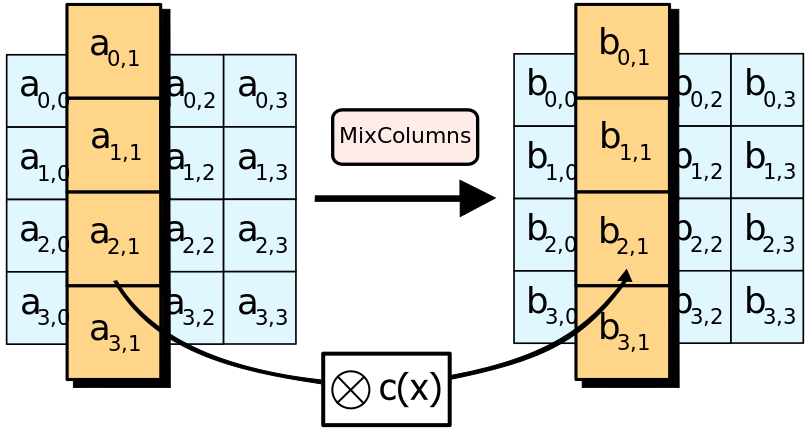
\includegraphics[width=0.6\textwidth]{capitoli/figure-crittografia/aes-MixColumns.png}
    \caption{Schema dell'operazione \emph{MixColumns}}
    \label{fig:aes-mixcolumns}
\end{figure}

\subsubsection{AddRoundKey}
Lo scopo di questa operazione è quella di combinare il blocco con la chiave del round, una chiave avente la stessa lunghezza del blocco e ottenuta a partire dalla \textbf{chiave di cifratura} utilizzata. In pratica la chiave di round viene organizzata nello stesso modo di un blocco e su ogni cella viene effettuato lo \emph{XOR} tra cella del blocco e cella della chiave di round. Una visualizzazione dell'operazione può essere vista in \autoref{fig:aes-addroundkey}. \cite{wikipedia_aes}

\begin{figure}[h]
    \centering
    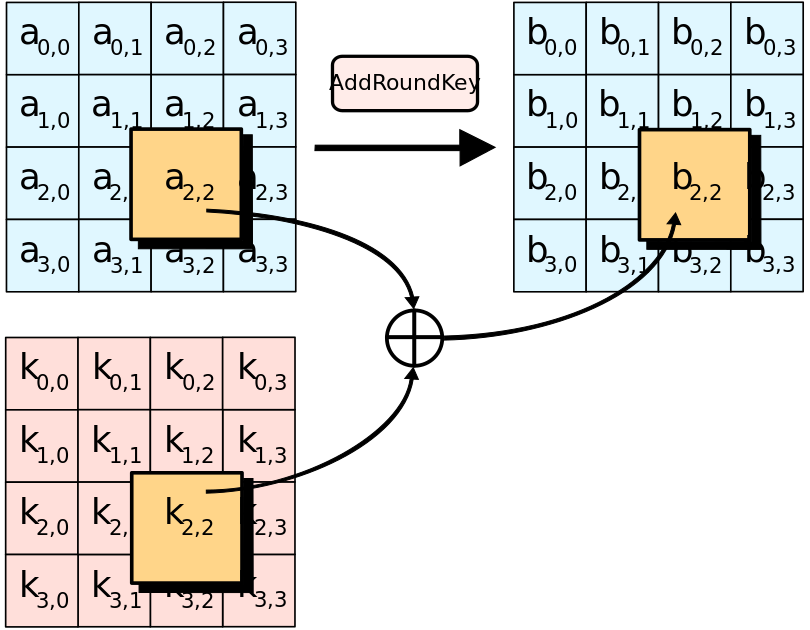
\includegraphics[width=0.6\textwidth]{capitoli/figure-crittografia/aes-AddRoundKey.png}
    \caption{Schema dell'operazione \emph{AddRoundKey}}
    \label{fig:aes-addroundkey}
\end{figure}

\subsection{Modalità di \emph{AES}} \label{section:aes-modes}
Essendo un cifrario a blocchi, opera su un dato preso in input blocco per blocco. Sebbene l'elaborazione di un singolo blocco è uguale per ognuno dal momento che l'algoritmo applicato è sempre uguale, lo stesso non vale per un gruppo consecutivo di blocchi in quanto questi possono essere elaborati in maniera diversa fornendo risultati completamente diversi. Si parla quindi di \textbf{modalità operative}, ovvero del modo in cui il cifrario elabora un input composto da più blocchi e le più diffuse sono le seguenti:

\begin{figure}[h]
    \centering
    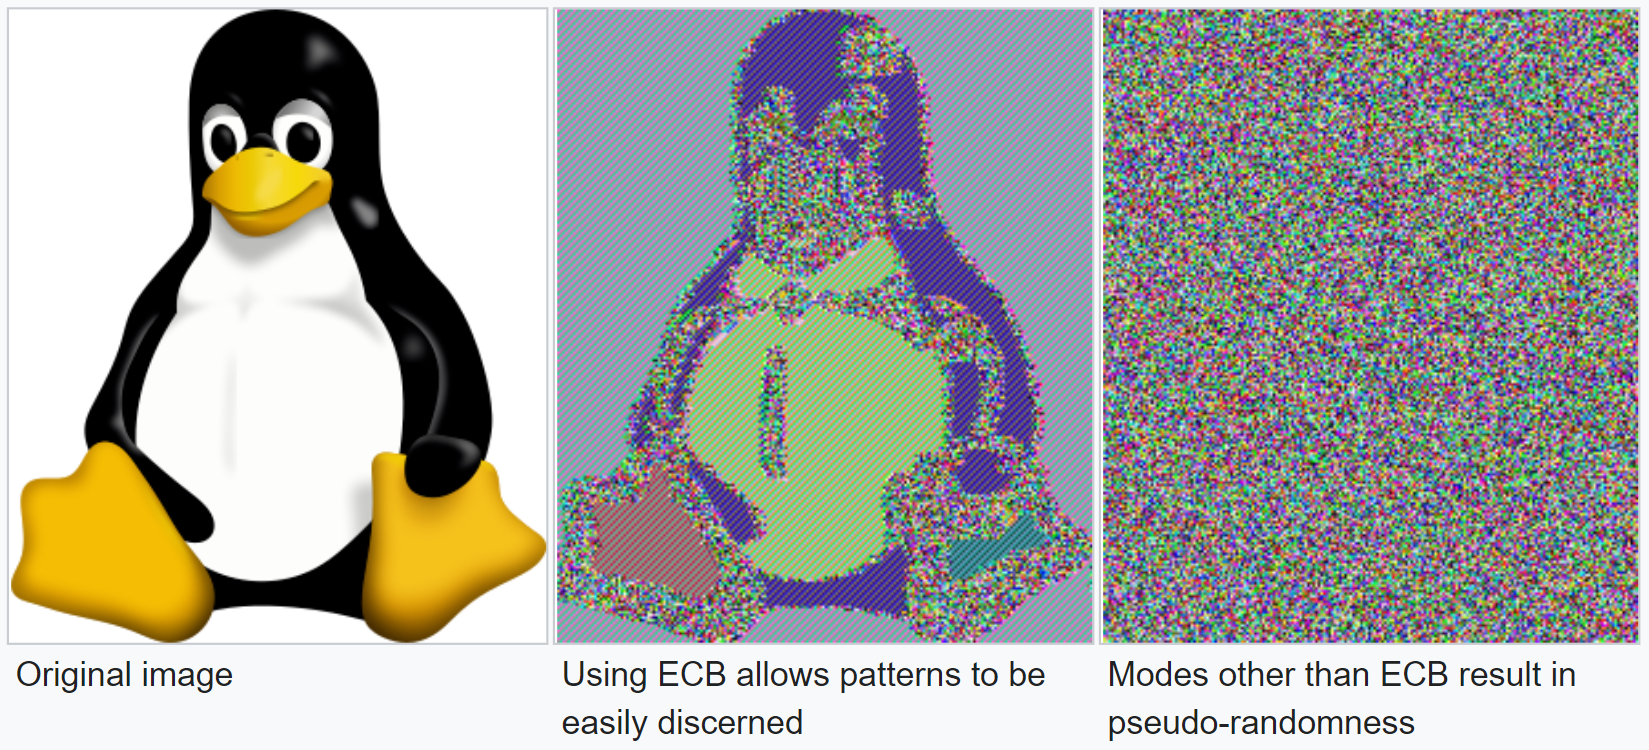
\includegraphics[width=0.6\textwidth]{capitoli/figure-crittografia/aes-ecb-linux.png}
    \caption{Problema con l'utilizzo della modalità \emph{ECB}}
    \label{fig:aes-ecb-linux}
\end{figure}


\begin{figure}[h!b]
    \begin{subfigure}{0.48\textwidth}
        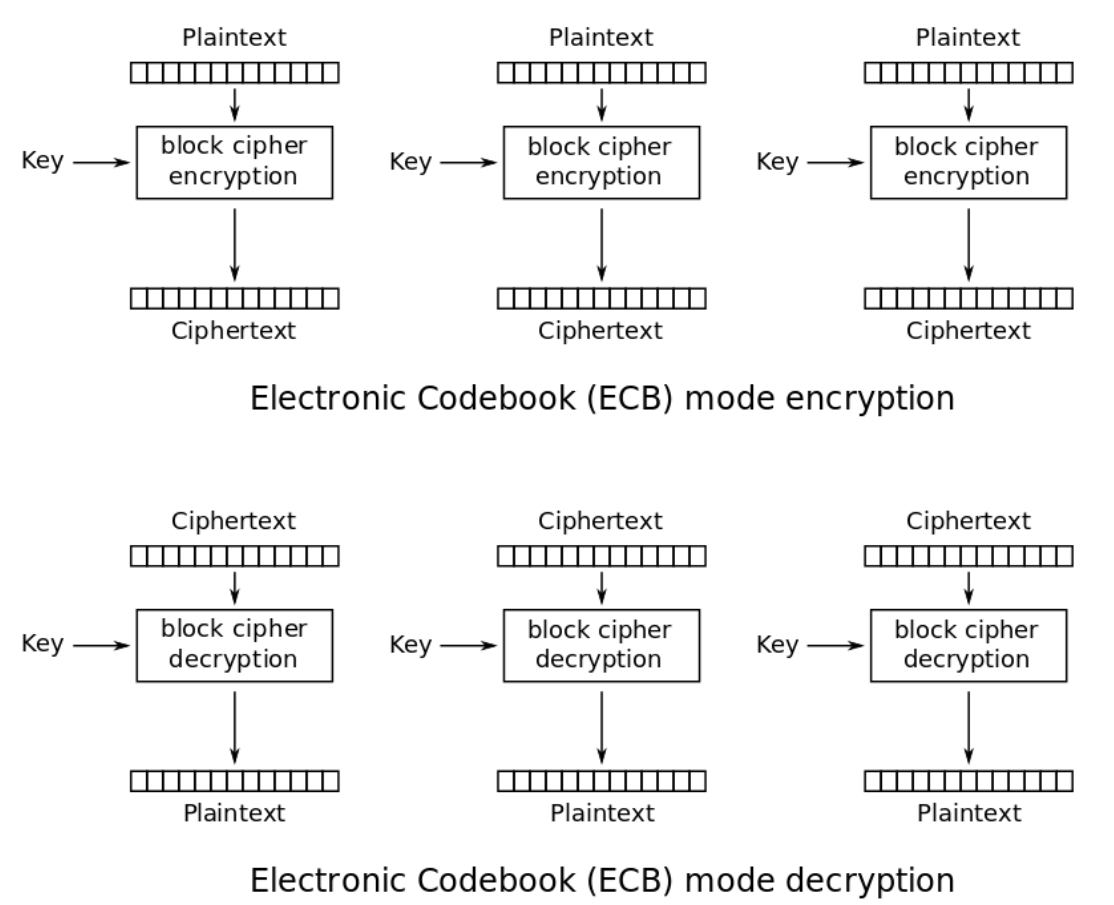
\includegraphics[width=1\textwidth]{capitoli/figure-crittografia/aes-ecb.png}
        \caption{Schema di funzionamento della modalità \emph{ECB}}
        \label{fig:aes-ecb}
    \end{subfigure}
    \begin{subfigure}{0.48\textwidth}
        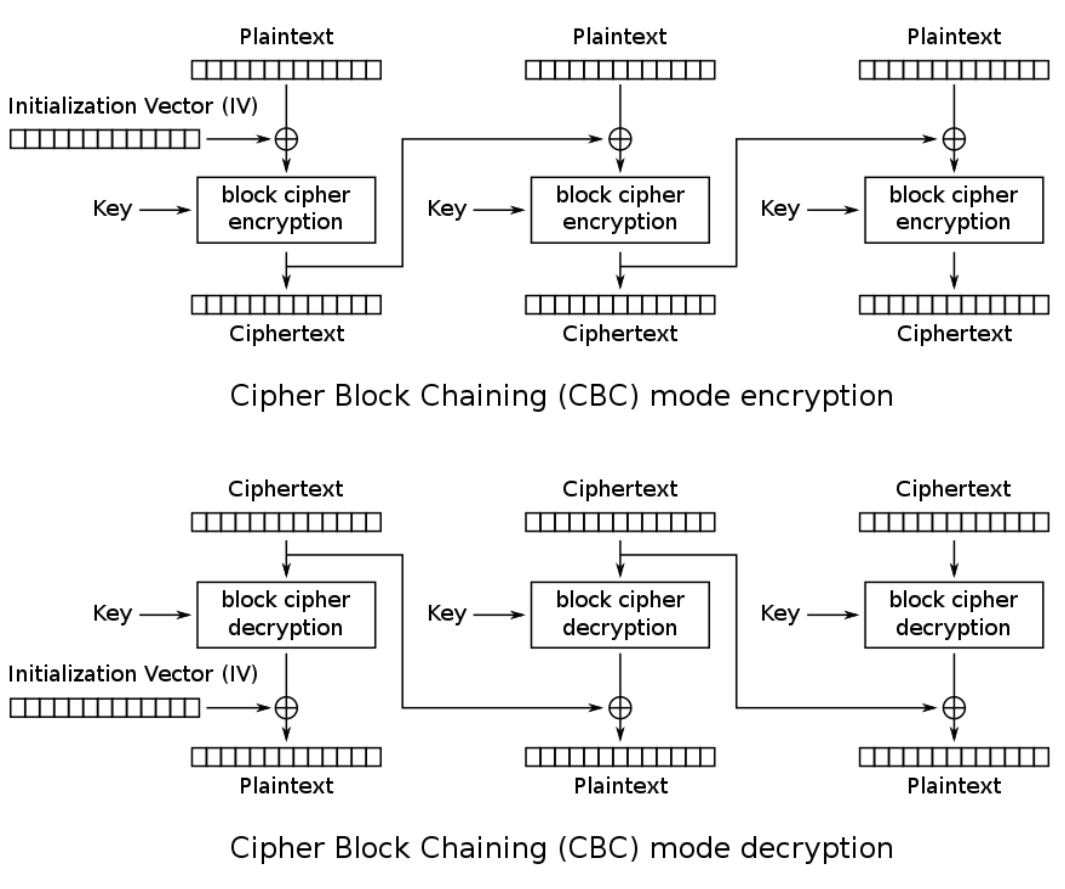
\includegraphics[width=1\textwidth]{capitoli/figure-crittografia/aes-cbc.png}
        \caption{Schema di funzionamento della modalità \emph{CBC}}
        \label{fig:aes-cbc}
    \end{subfigure}
    \begin{subfigure}{0.48\textwidth}
        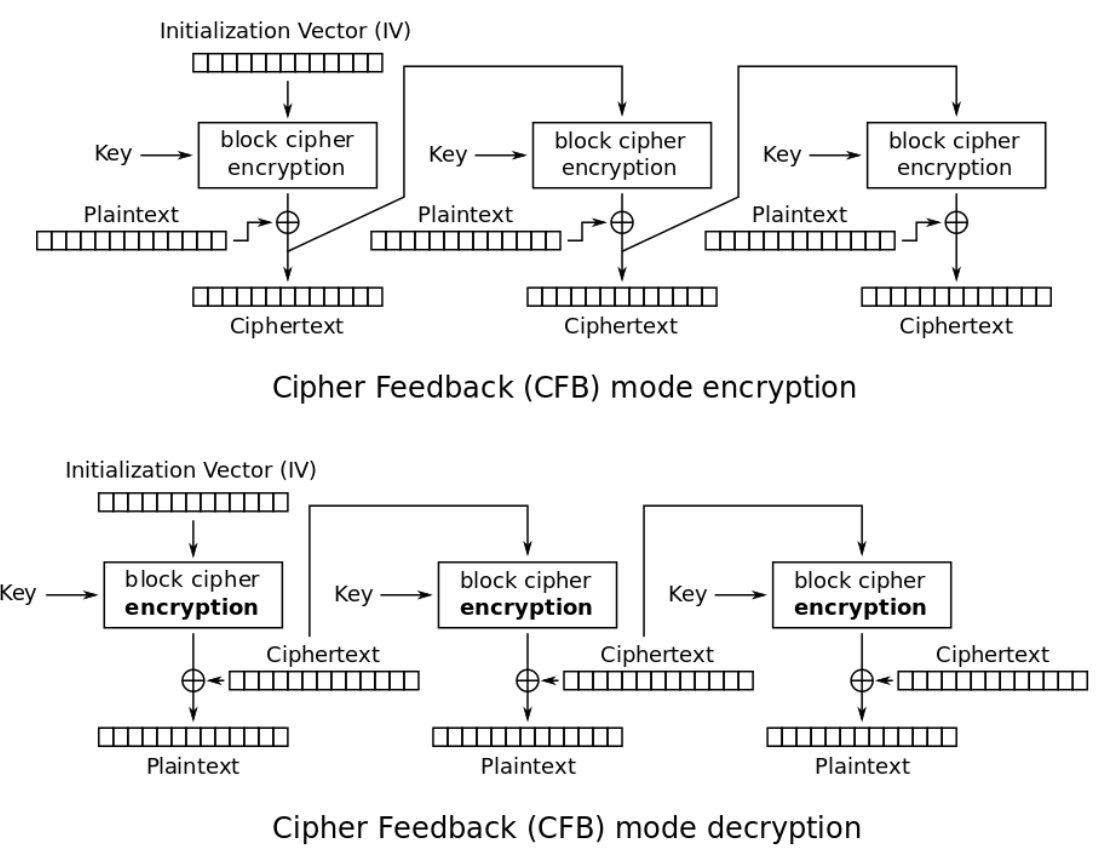
\includegraphics[width=1\textwidth]{capitoli/figure-crittografia/aes-cfb.png}
        \caption{Schema di funzionamento della modalità \emph{CFB}}
        \label{fig:aes-cfb}
    \end{subfigure}
    \begin{subfigure}{0.48\textwidth}
        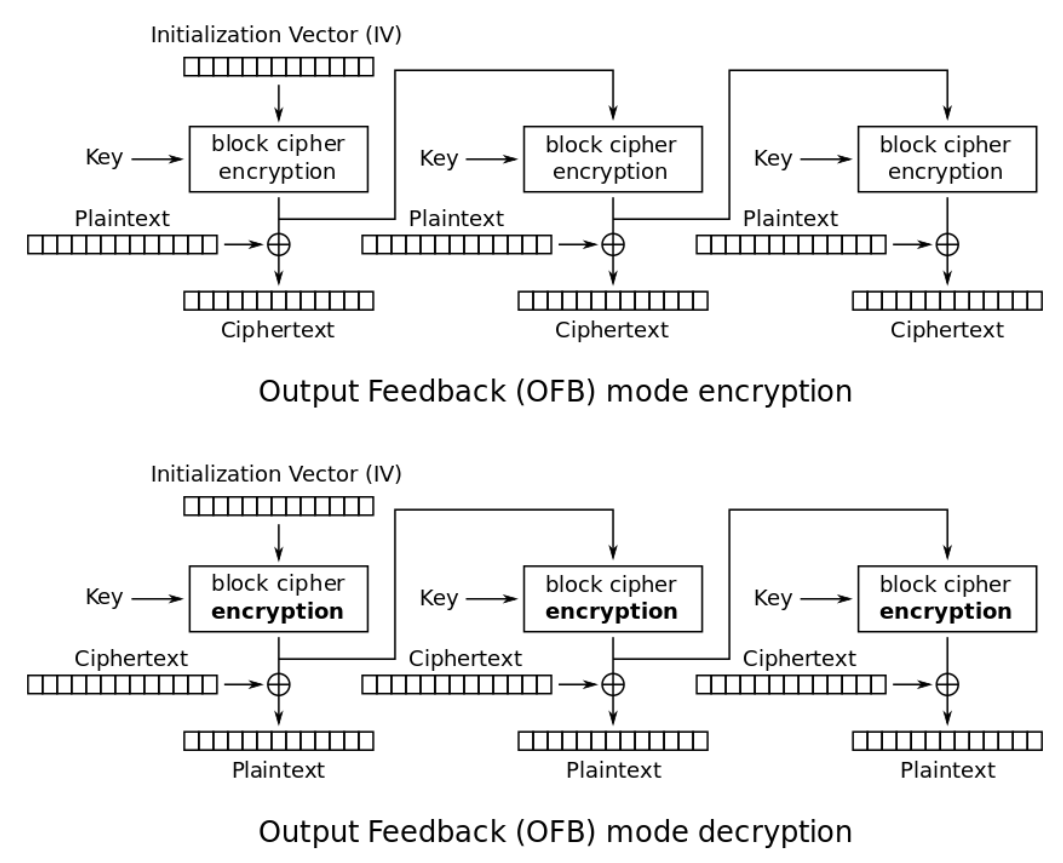
\includegraphics[width=1\textwidth]{capitoli/figure-crittografia/aes-ofb.png}
        \caption{Schema di funzionamento della modalità \emph{OFB}}
        \label{fig:aes-ofb}
    \end{subfigure}
    \centering
    \begin{subfigure}{0.48\textwidth}
        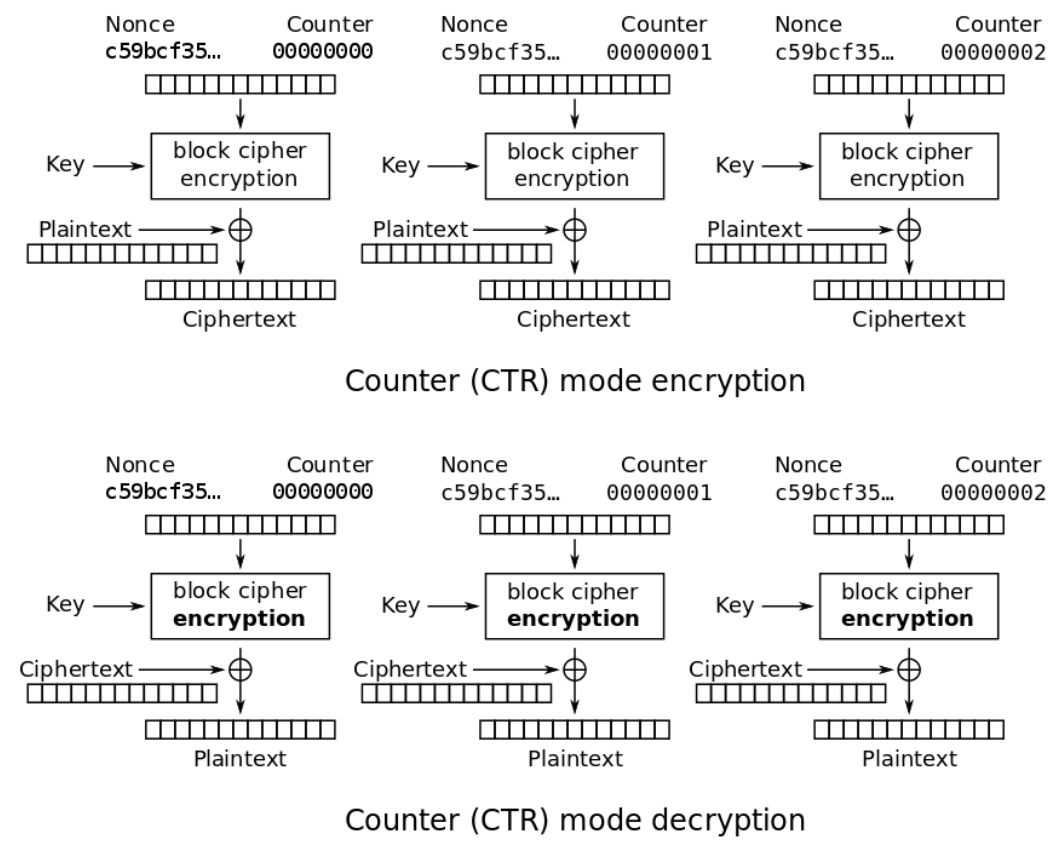
\includegraphics[width=1\textwidth]{capitoli/figure-crittografia/aes-ctr.png}
        \caption{Schema di funzionamento della modalità \emph{CTR}}
        \label{fig:aes-ctr}
    \end{subfigure}
    \caption{Modalità operative di \emph{AES}}
    \label{fig:aes-modes}
\end{figure}

\begin{itemize}
    \item \textbf{ECB} (Electronic Codebook): modalità più semplice dove ogni blocco viene elaborato in maniera indipendente. Non più utilizzato in quanto codificando uno stesso \emph{testo in chiaro} sempre con lo stesso \emph{testo cifrato}, non nasconde bene i pattern e manca di \textbf{diffusione}. Uno schema che descrive il funzionamento si trova in \autoref{fig:aes-ecb} mentre un esempio che mostra il problema evidenziato si trova in \autoref{fig:aes-ecb-linux};
    \item \textbf{CBC} (Cipher Block Chaining): modalità in cui ogni blocco contribuisce all'elaborazione del blocco successivo. In pratica, nel caso della cifratura, il testo cifrato ottenuto dal blocco precedente viene messo in \emph{XOR} con il blocco attuale e il risultato viene dato in pasto alla cifratura mentre, nel caso della decifratura, il testo cifrato precedente viene messo in \emph{XOR} con l'output della decifratura per ottenere il testo in chiaro. Essendo che per il primo blocco non esiste un blocco precedente, viene usato un blocco predefinito e noto chiamato \textbf{vettore di inizializzazione} che non fa parte dell'input ma viene aggiunto. Uno schema che descrive il funzionamento si trova in \autoref{fig:aes-cbc};
    \item \textbf{CFB} (Cipher Feedback): modalità molto simile alla \emph{CBC}, dove nel caso della cifratura il testo in chiaro viene messo in \emph{XOR} con l'output dello \emph{XOR} tra cifratura del blocco precedente e testo in chiaro precedente per ottenere il testo cifrato, mentre nel caso della decifratura il testo cifrato viene messo in \emph{XOR} con l'output della \textbf{cifratura} del blocco precedente. Anche in questo caso è necessario un \textbf{vettore di inizializzazione} e uno schema che descrive il funzionamento si trova in \autoref{fig:aes-cfb};
    \item \textbf{OFB} (Output Feedback): modalità dove nel caso della cifratura il testo in chiaro viene messo in \emph{XOR} con l'output della cifratura del blocco precedente per ottenere il testo cifrato, mentre nel caso della decifratura l testo cifrato viene messo in \emph{XOR} con l'output della \textbf{cifratura} del blocco precedente per ottenere il testo in chiaro. Anche in questo caso è necessario un \textbf{vettore di inizializzazione} e uno schema che descrive il funzionamento si trova in \autoref{fig:aes-ofb}.
    \item \textbf{CTR} (Counter): modalità dove i blocchi vegono elaborati in maniera indipendente (simile a \emph{ECB}). Per prima cosa viene generato un \textbf{nonce} (un numero casuale) al quale viene sommato un contatore che parte da 0 e viene incrementato man mano che si processano i blocchi. Il valore ottenuto viene dato in pasto alla cifratura e il risultato viene messo in \emph{XOR} con il blocco per ottenere il testo cifrato. Anche nel caso della decifratura il risultato della somma viene dato in input alla \textbf{cifratura}, ma questo viene messo in \emph{XOR} con il testo cifrato per ottenere il testo in chiaro. Uno schema che descrive il funzionamento si trova in \autoref{fig:aes-ctr}. \cite{wikipedia_aes_modes}
\end{itemize}

Un confronto che si può fare tra le varie modalità riguarda la possibilità di parallelizzare cifratura e decifratura e la possibilità di effettuare l'accesso casuale in lettura ad un blocco dell'input. Una tabella riassuntiva di tale confronto può essere consultato in \autoref{table:aes-modes-comparison} \cite{wikipedia_aes_modes}

\begin{table}[h]
    \centering
    \begin{tabular}[h]{| c || c | c | c | c | c |}
        \hline
        \textbf{Modalità} & \textbf{ECB} & \textbf{CBC} & \textbf{CFB} & \textbf{OFB} & \textbf{CTR} \\
        \hline
        \textbf{Cifratura parallelizzabile?} & si & no & no & no & si \\
        \hline
        \textbf{Decifratura parallelizzabile?} & si & si & si & no & si \\
        \hline
        \textbf{Accesso casuale} & si & si & si & no & si \\
        \hline
    \end{tabular}
    \caption{Confronto tra le varie modalità operative}
    \label{table:aes-modes-comparison}
\end{table}

\subsection{Sicurezza del cifrario}
Un algoritmo di cifratura è considerato sicuro se il miglior algoritmo utilizzabile per "romperlo" è l'algortimo di \textbf{forza bruta}, ovvero vengono provate tutte le possibili chiavi in sequenza fino ad indovinare quella corretta. \emph{AES}, fino ad oggi, è ancora considerato sicuro in quanto non è stato ancora trovato nessun attacco realizzabile nei suoi confronti anche se sono stati \textbf{teorizzati} dei possibili attacchi. Uno degli attacchi più famosi in letteratura è chiamato \textbf{XSL Attack} (eXtended Sparse Linearization), il quale cerca di sfruttare una debolezza di \emph{AES} dovuta alla scarsa complessità delle componenti \textbf{non lineari} ma è stato dimostrato che questo attacco non è praticabile, quindi rimane sicuro anche rispetto a questo attacco. Un altro attacco molto famoso è l'attacco \textbf{biclique}, una variante del \textbf{Meet-In-The-Middle} (un attacco che sfrutta combinazioni di testi in chiaro e cifrati per ricavare la chiave di cifratura) che è stato dimostrato essere 4 volte più veloce di un attacco a forza bruta. Tuttavia, analizzando il guadagno ottenuto in termini di \textbf{parametro di sicurezza} quello che si ottiene è che invece di ottenere una sicurezza a 128 bit (per \emph{AES-128}) si ottiene una sicurezza di 126 bit (2 bit in meno anche per le altre varianti di \emph{AES}), che è ancora un ottimo livello di sicurezza in quanto per concludere con successo un attacco del genere sono ancora richiesti \textbf{miliardi di anni}. Quindi anche nei confronti di quest'ultimo attacco è considerato ancora sicuro. \cite{wikipedia_aes}

Inoltre, è stato recentemente dimostrato che \emph{AES} è anche \textbf{Quantum-safe} ed è quindi persino in grado di resistere ad un attacco di un computer quantistico. Ovviamente, essendo più potente, il livello di sicurezza offerto dalle varie versioni dell'algoritmo sarà minore rispetto a quelle offerte per i computer classici. Un confronto, in termini di livello di sicurezza offerto, tra computer classici e quantistici può essere visto in \autoref{table:aes-security}. \cite{aes_quantum_safe}

\begin{table}[h]
    \centering
    \begin{tabular}{| c | c | c | c |}
        \hline
        \textbf{Algoritmo} & \textbf{Lunghezza chiave} & \textbf{Sicurezza classica} &\textbf{Sicurezza quantum} \\
        \hline
        AES-128 & 128 bit & 128 bit & 64 bit \\
        \hline
        AES-256 & 256 bit & 256 bit & 128 bit \\
        \hline
    \end{tabular}
    \caption{Sicurezza offerta da \emph{AES} per computer classici e quantistici}
    \label{table:aes-security}
\end{table}

\newpage